\documentclass[tikz,border=12pt]{standalone}
\usepackage{amsmath}
\usetikzlibrary{arrows.meta,calc}

\begin{document}
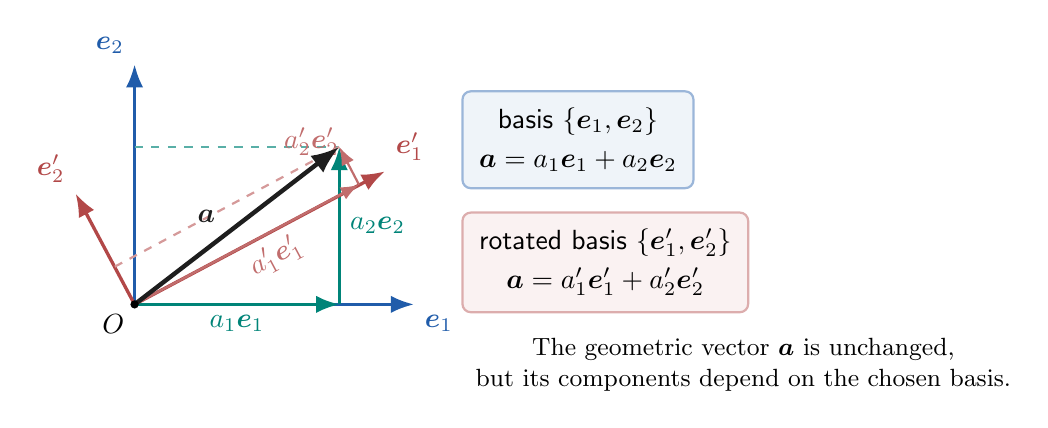
\begin{tikzpicture}[>=Latex,font=\sffamily,thick]
\definecolor{basis}{RGB}{32,92,170}
\definecolor{rotbasis}{RGB}{178,72,72}
\definecolor{vector}{RGB}{30,30,30}
\definecolor{component}{RGB}{0,132,120}

\coordinate (O) at (0,0);
\coordinate (A) at (2.60,2.00);
\coordinate (P) at (2.85,1.52);

% Original orthonormal basis.
\draw[->,basis,very thick] (O)--(3.55,0)
  node[below right] {$\boldsymbol e_1$};
\draw[->,basis,very thick] (O)--(0,3.05)
  node[above left] {$\boldsymbol e_2$};

% Components in the original basis.
\draw[->,component,very thick] (O)--(2.60,0)
  node[midway,below] {$a_1\boldsymbol e_1$};
\draw[->,component,very thick] (2.60,0)--(A)
  node[midway,right] {$a_2\boldsymbol e_2$};
\draw[dashed,component!65] (0,2.00)--(A);

% Rotated basis and its component parallelogram.
\draw[->,rotbasis,very thick] (O)--(3.18,1.69)
  node[above right] {$\boldsymbol e'_1$};
\draw[->,rotbasis,very thick] (O)--(-0.75,1.41)
  node[above left] {$\boldsymbol e'_2$};
\draw[->,rotbasis!80,thick] (O)--(P)
  node[pos=0.58,below,sloped] {$a'_1\boldsymbol e'_1$};
\draw[->,rotbasis!80,thick] (P)--(A)
  node[midway,above left] {$a'_2\boldsymbol e'_2$};
\draw[dashed,rotbasis!55] (-0.25,0.48)--(A);

% Physical vector, drawn last.
\draw[->,vector,ultra thick] (O)--(A)
  node[pos=0.45,above left] {$\boldsymbol a$};
\fill (O) circle (1.5pt) node[below left] {$O$};

% Explanatory boxes.
\node[draw=basis!45,fill=basis!7,rounded corners=3pt,align=center,
      inner sep=6pt,anchor=north west] at (4.15,2.72)
  {basis $\{\boldsymbol e_1,\boldsymbol e_2\}$\\[2pt]
   $\boldsymbol a=a_1\boldsymbol e_1+a_2\boldsymbol e_2$};
\node[draw=rotbasis!45,fill=rotbasis!7,rounded corners=3pt,align=center,
      inner sep=6pt,anchor=north west] at (4.15,1.18)
  {rotated basis $\{\boldsymbol e'_1,\boldsymbol e'_2\}$\\[2pt]
   $\boldsymbol a=a'_1\boldsymbol e'_1+a'_2\boldsymbol e'_2$};
\node[align=center,font=\small,anchor=north west] at (4.20,-0.30)
  {The geometric vector $\boldsymbol a$ is unchanged,\\
   but its components depend on the chosen basis.};

\end{tikzpicture}
\end{document}
